%% Based on a TeXnicCenter-Template, which was
%% created by Christoph B�rensen
%% and slightly modified by Tino Weinkauf.
%%%%%%%%%%%%%%%%%%%%%%%%%%%%%%%%%%%%%%%%%%%%%%%%%%%%%%%%%%%%%

\documentclass[a4paper,12pt]{scrartcl} %This is a special class provided by the KOMA script, which does a lot of adjustments to adapt the standard LaTeX classes to european habits, change to [a4paper,12pt,twoside] for doublesided layout


%########################### Preferences #################################


% ******** vmargin settings *********
\usepackage{vmargin} %This give you full control over the used page arae, it maybe not the idea od Latex to do so, but I wanted to reduce to amount of white space on the page
\setpapersize{A4}
\setmargins{3.5cm}%			%linker Rand, left edge
					 {1.5cm}%     %oberer Rand, top edge
           {14.7cm}%		%Textbreite, text width
           {23.42cm}%   %Texthoehe, text hight
           {14pt}%			%Kopfzeilenh�he, header hight
           {1cm}%   	  %Kopfzeilenabstand, header distance
           {0pt}%				%Fu�zeilenhoehe footer hight
           {2cm}%    	  %Fusszeilenabstand, footer distance         

% ********* Font definiton ************
\usepackage{t1enc} % as usual
\usepackage[latin1]{inputenc} % as usual
\usepackage{times}		
%\usepackage{mathptmx}  	%mathematical fonts for use with times, I encountered some problems using this package togather with pdftex, which I was not able to resolve

% ********* Graphics definition *******
\usepackage[pdftex]{graphicx} % required to import graphic files
\usepackage{color} %allows to mark some entries in the tables with color
\usepackage{eso-pic} % these two are required to add the little picture on top of every page
\usepackage{everyshi} % these two are required to add the little picture on top of every page
\renewcommand{\floatpagefraction}{0.7} %default:0.5 allows two big pictures on one page

%********** Enybeling Hyperlinks *******
\usepackage[pdfborder=000,pdftex=true]{hyperref}% this enables jumping from a reference and table of content in the pdf file to its target

% ********* Table layout **************
\usepackage{booktabs}	  	%design of table, has an excellent documentation
%\usepackage{lscape}			%use this if you want to rotate the table together with the lines around the table

% ********* Caption Layout ************
\usepackage{ccaption} % allows special formating of the captions
\captionnamefont{\bf\footnotesize\sffamily} % defines the font of the caption name (e.g. Figure: or Table:)
\captiontitlefont{\footnotesize\sffamily} % defines the font of the caption text (same as above, but not bold)
\setlength{\abovecaptionskip}{0mm} %lowers the distace of captions to the figure


% ********* Header and Footer **********
% This is something to play with forever. I use here the advanced settings of the KOMA script

\usepackage{scrpage2} %header and footer using the options for the KOMA script
\renewcommand{\headfont}{\footnotesize\sffamily} % font for the header
\renewcommand{\pnumfont}{\footnotesize\sffamily} % font for the pagenumbers

%the following lines define the pagestyle for the main document
\defpagestyle{cb}{%
(\textwidth,0pt)% sets the border line above the header
{\pagemark\hfill\headmark\hfill}% doublesided, left page
{\hfill\headmark\hfill\pagemark}% doublesided, right page
{\hfill\headmark\hfill\pagemark}%  onesided
(\textwidth,1pt)}% sets the border line below the header
%
{(\textwidth,1pt)% sets the border line above the footer
{{\it University of Central Lancashire}\hfill QHong}% doublesided, left page
{QHong\hfill{\it University of Central Lancashire}}% doublesided, right page
{QHong\hfill{\it University of Central Lancashire}} % one sided printing
(\textwidth,0pt)% sets the border line below the footer
}

%this defines the page style for the first pages: all empty
\renewpagestyle{plain}%
	{(\textwidth,0pt)%
		{\hfill}{\hfill}{\hfill}%
	(\textwidth,0pt)}%
	{(\textwidth,0pt)%	
		{\hfill}{\hfill}{\hfill}%
	(\textwidth,0pt)}

%********** Footnotes **********
\renewcommand{\footnoterule}{\rule{5cm}{0.2mm} \vspace{0.3cm}} %increases the distance of footnotes from the text
\deffootnote[1em]{1em}{1em}{\textsuperscript{\normalfont\thefootnotemark}} %some moe formattion on footnotes

%################ End Preferences, Begin Document #####################

\pagestyle{plain} % on headers or footers on the first page

\begin{document}

\begin{center}

\begin{figure}[th]
    \centering
		%\includegraphics[width=10cm]{logo.jpg}
	\label{fig:logo}
\end{figure}

\vspace{2cm}

% There might be better solutions for the title page, giving all distances and sizes manually was simply the easiest solution

{\Huge\bf\sf Report for a }

\vspace{.5cm}

{\Huge\bf\sf Monthly Meeting}

\vspace{.5cm}

{\Huge\bf\sf }

\vspace{2cm}

{\Large\bf\sf Hong, Q.}%as this is an english text I didn't load the german package, this would ease the use of special characters
\vspace{2cm}

{\Large\bf\sf Supervisor Team : }
\vspace{2cm}

{\Large\bf\sf                   Platt, S.P. ~\\}
\vspace{2cm}
{\Large\bf\sf                   Mein, S.J.}
\vspace{2cm}

{\Large\bf\sf \today} %adds the current date

\vspace{2cm}
{\Large\bf\sf University of Central Lancashire}

\vspace{\fill}

qhong@uclan.ac.uk

\end{center}
\newpage

%%The following loads the picture on top of every page, the numbers in \put() define the position on the page:
%\AddToShipoutPicture{\setlength\unitlength{0.1mm}\put(604,2522){\includegraphics[width=1.5cm]{logo.jpg}}}

\pagestyle{cb} % now we want to have headers and footers

\tableofcontents

\newpage
\section{Project Background}
Single event effect have an impact on electronic devices, especially applied in outer space, aircraft altitude and terrestrial environment. On the sea level, neutron as one of the factors induced single event effect has received attentions since Ziegler found soft fails in computer electronics \cite{5389432}. Testing single event effect on electronic devices under natural neutron fields is not only expensive but also time consuming. Using accelerated neutron Single Event Effect (SEE) testing to explore SEE on electronic devices and system is a well established technique. As the basis of simulation, two test facilities have been considered as simulation model in the project, one is LANSCE ICE House and the other is The Svedberg Laboratory (TSL) \cite{5488795,5173383}.
% Advantages of accelerated testing including: (1) Environment conditions can be controlled by human being. (2) We can choose the type and energy of the particle so that it is good for all respects of research on SEE. (3) The experiment is not only repeatable but also for a study with a single factor. It is important to explore the mechanism of single event effect.
The silicon photodiodes have been applied in local beam monioring for accelerated neutron SEE testing is used to obtain a reliable estimation of neutron induced SEE cross-section \cite{6131336}. It has been found that there is a possibility of gamma rays deposited energy in the photodiodes \cite{ZhangThesis}. Monte Carlo simulation is good for quantitative analysis of physical and mathematical problems. The Geant4 software toolkit as a open source is developed for the passage of particles through the matter. 
% The experiments can be carried out with several testing sets arraged along a beam line. In such case, devieces that are positioned further away from the beam source receive a degraded beam due to absorption and scattering by upstream experiments. The consequent loss of neutron fluence cannot be accounted for by typical upstream beam monitoring. In order to make reliable estimation of SEE cross-section. Local Beam Monitoring are necessary.

My project is going to use Geant4 toolkit to simulate accelerated neutron SEE testing(LANSCE and TSL), calculate neutron and gamma flux at different positions along the beam line, and compare to existing database of neutron flux.

\section{Current Plan}

Compare LANSCE measurement results with Geant4 simulation results, it shows the simulated neutron flux is a little bit higher than measurement results below about 10{MeV}. It is considered to attach collimator to take a look.

\subsection{LANSCE results comparison}
Comparison of neutron flux of LANSCE measurement results and Geant4 simulation results at 30 degree with collimator attached. 
Comparison of neutron flux of LANSCE calculation results and Geant4 simulation results at 30 degree with collimator attached. 

\subsection{ANITA results comparison}
Comparison of neutron flux of analytical ANITA results and Geant4 simulation results at 0 degree with collimator attached. 

\subsection{Simulation results comparison}
Comparison neutron flux  of Geant4 simulation results at 0 (or 15, 30, 60 90) degree  without collimator attached and with collimator attached under Bertini Model.

Comparison neutron flux  of Geant4 simulation results at 0 (or 15, 30, 60 90) degree  without collimator attached and with collimator attached under Binary Model.

Comparison gamma flux  of Geant4 simulation results at 0 (or 15, 30, 60 90) degree  without collimator attached and with collimator attached under Bertini Model.

Comparison gamma flux  of Geant4 simulation results at 0 (or 15, 30, 60 90) degree  without collimator attached and with collimator attached under Binary Model.


To implement these plans, it needs to construct the collimator in the geometry and place two more detectors in tandem of the collimator. Then it is possible to calculate neutron (gamma) deposition parameters in collimator, for example, neutron (gamma) fluence. 

\section{Progress against the plan}

Construction of collimator does not go well. Only neutron detectors are attached in the codes. Gamma detectors will be established in Geometry. 

No source management for this project, no records for the changes in each time. 

\section{Achievements since last meeting}

\subsection{Geometry of collimator}
It shows positions of neutron source, detectors and collimator in accelerate SEE testing at The Svedberg Laboratory (TSL) \cite{5336295}. This collimator is made up steel cuboid with a hole of 102{mm} in diameter. Reference to Figure \ref{fig:view}. As it shows, some of neutrons could pass through the middle of the hole, some would go back and some have been stopped by collimator. 

\begin{figure*}[ht]\centering % Using \begin{figure*} makes the figure take up the entire width of the page
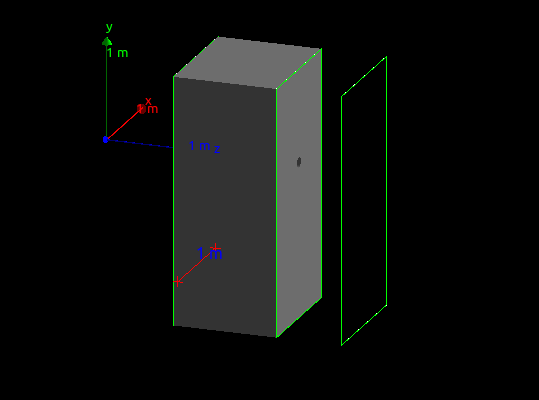
\includegraphics[width=\linewidth]{Geometry}
\caption{Geometry with collimator append}
\label{fig:view}
\end{figure*}

\subsection{Position of detectors}
In order to compare the neutron fluence results with and without adding collimator. Two more detectors will be attached along the incident direction of proton (+z) to calculate neutrons. They are located (0,0,867{mm}) , (0,0,collimatorLength + 867{mm}) and (0,0,2.5{m}) respectively to calculate neutrons before the neutron passing through the collimator, after the passage of neutron through the collimator. The third detector is placed in Standard User Position (it existed in the previous simulation, no collimator constructed)\cite{5336295}. The output file should contain more information, like detector ID.
% Downstream of production target Standard User Position

\subsection{Getting Started - Git}
Git is a good tool used as source manager to record changes and restore the project programming so that it is easy to recall any version at anytime anywhere. This version control system now is going to record any changes of this project. The git is used to store the snapshots for each time which is different from other competing product such as subversion. Commit, which takes the files as they are in the staging area and stores that snapshot permanently to your Git directory. Push, which takes the database from Git directory to another repository \cite{gitManual}. The following Figure\ref{fig:gitview} shows a Git on server.

\begin{figure*}[ht]\centering % Using \begin{figure*} makes the figure take up the entire width of the page
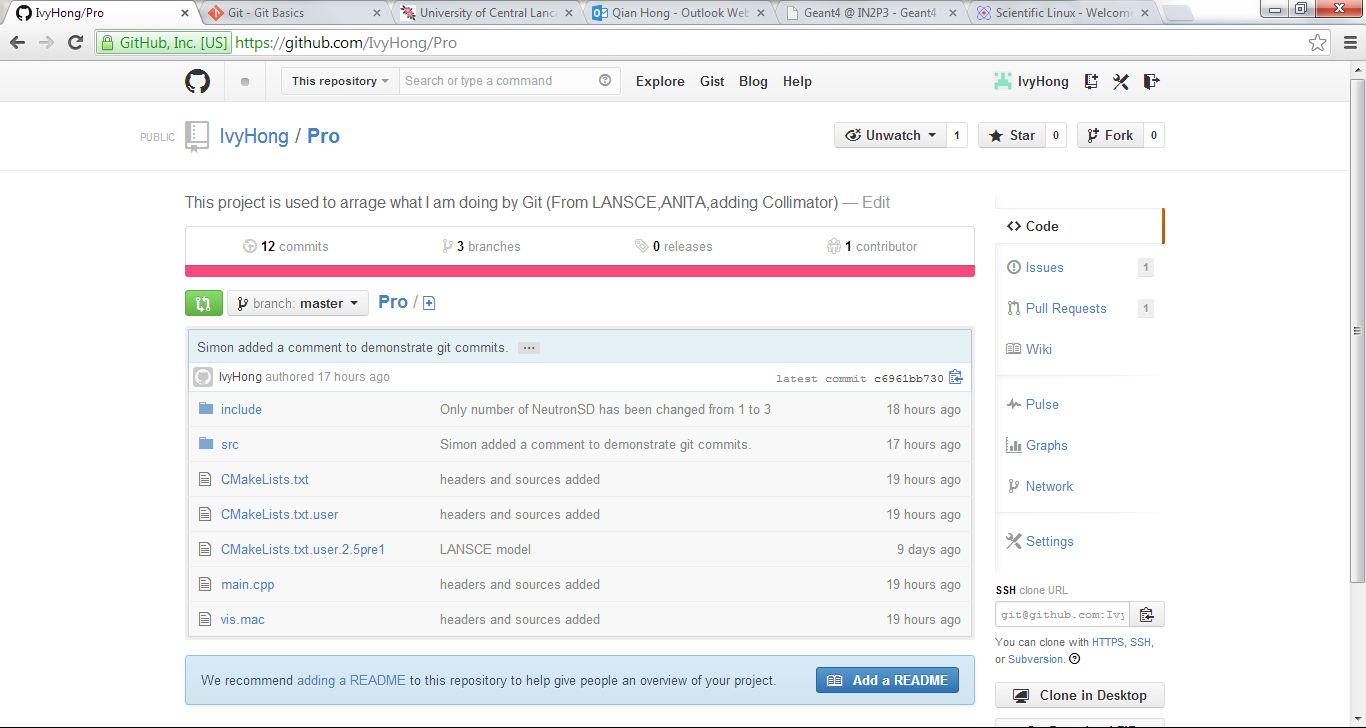
\includegraphics[width=\linewidth]{Gitview}
\caption{Git Repository}
\label{fig:gitview}
\end{figure*}

% Version control. Git, every time you commit, or save the state of your project in Git, it basically takes a picture of what all your files look like at that moment and stores a reference to that snapshot.
% Git has three main states that your files can reside in: committed, modified, and staged. Committed means that the data is safely stored in your local database. Modified means that you have changed the file but have not committed it to your database yet. Staged means that you have marked a modified file in its current version to go into your next commit snapshot. This leads us to the three main sections of a Git project: the Git directory, the working directory, and the staging area.

%\subsubsection{}
\subsection{G4 Learning}

The visualization can be controlled from both commands and compiled code. The commands are written in macro file withe using commands like /vis/open "visualization driver" and /vis/drawVolume. 
% /vis/open creates a scene handler and viewer
% create an empty scene
% /vis/drawVolume add physical volume to the scene,default is world
% Commands in the command directory "/vis/viewer/" set camera parameters and drawing style of the current
Visualization Manager G4VVisManager, which as calling methods existing in G4UserRunAction and G4UserEventAction so that when Geant4 simulation is running, visualization can be implement with no user intervention .
% G4VVisManager::Draw()

\subsection{Geant4 Installation support}

New finding for Geant4, Geant4 is officially supported on Scientific Linux CERN 5 with gcc 4.1.2 or 4.3.X, 32/64bit and Scientific Linux CERN 6 with gcc 4.6.X, 64bit. This operating system has been installed, the following Figure\ref{fig:SL6view} shows interface. It is possible to try this system rather than one system. Now Geant4 source code has been installed in SL6 but lack of Integrated development environment. XCode and Eclipse are suggested in Geant4 installation manual and it is precious to try. 

\begin{figure*}[ht]\centering % Using \begin{figure*} makes the figure take up the entire width of the page
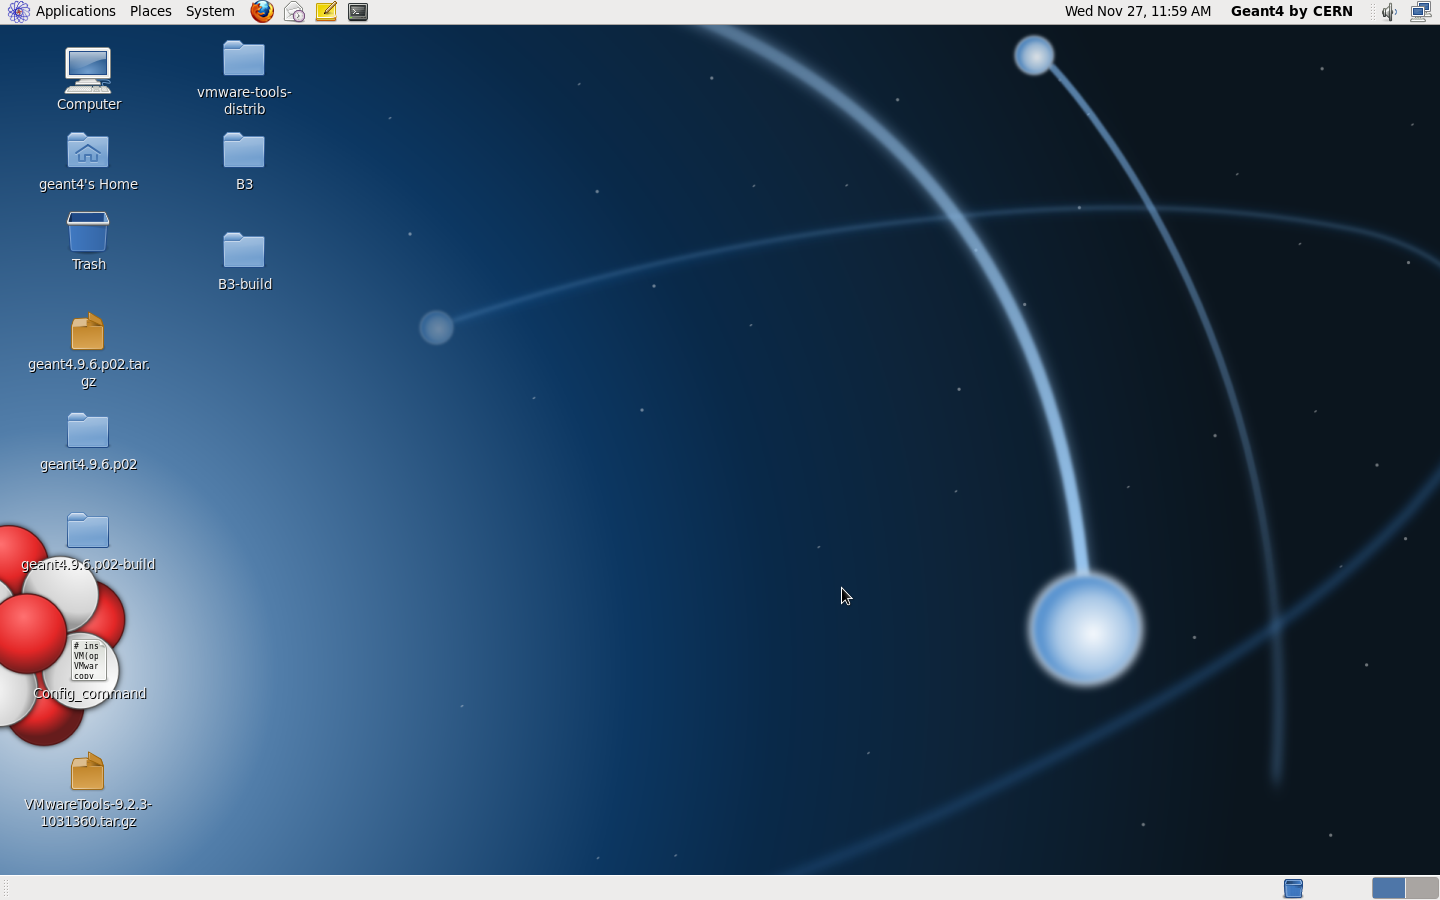
\includegraphics[width=\linewidth]{SL6}
\caption{Scientific Linux Operating system user interface}
\label{fig:SL6view}
\end{figure*}

\subsection{Latex}
Using text editor (TexnicCenter) to write monthly meeting report.

\section{Difficulties encounted since last meeting}
\subsection{Problem.1}
Two detectors have been attached, no records from the output files. In order to check the programming, Debugger of Qt creator would be used, but it fails to debug. The commands existing in macro file which are not compatible with the Qt creator debugger.
\subsection{Problem.2}
Except for these, any source manager has not used in this PhD project. That will be a problem. No records for each modification. The program is unable to get back according to time.
\subsection{Problem.3}
The geometry of collimator seems not correct from visualization interface window. The hole does not penetrate the collimator.

\section{Next steps}
\subsection{Step.1}
Collimator geometry needs to be checked through minimal working example method. It is capable of creating a small project which used to check geometry. ~\\

After examination, if the problem can be sorted it out, the progress will follow the plan step by step.  
If the examination result is not ideal, it should be read Geant4 user manual and ask Supervisor for help \cite{geant4Manual}. 

\subsection{Step.2}
Doing research to find out Xcode and Eclipse in Linux and install on scientific Linux 6. If it works well, I would be familiar with using Geant4 in different system. 

\section{Actions}

Further aim is to submit a paper.

\section{Revised plan}

%----------------------------------------------------------------------------------------
%	REFERENCE LIST
%----------------------------------------------------------------------------------------

\bibliographystyle{unsrt}
\bibliography{MMRef}

%----------------------------------------------------------------------------------------

\end{document}

%\begin{landscape} %in case a table becomes to big this rotates it, uncheck also \end{landscape} and lscape package in the preferences
%	\begin{table}
%		\caption[Substrate matrix 1]{\rule[-2mm]{0mm}{0mm}{Physical properties of the tested substrate samples}}
%		\begin{tabular}{@{}*{8}l@{}} \toprule \addlinespace[0.1em]

%      No.  &  Supplier  &  Material  &    Sample  &    Length  &  Identifier  &      Mass  &       Mass \\

%           &            &            &            &       /cm  &              &      Mass  & /g$^{a)}$ \\

%\cmidrule{1-8} % &            &            &            &            &            &            &            \\

%         1 &        SST &     Galaxy &  warp unit &         15 &   \color{red}ncc1701e &     1927.6 &     1920.2 \\

%         2 &        SST & Constellat. &  warp unit &       14.9 &   11016910 &    ---     &    ---     \\

%         3 &        SST &  Prototype &        ops &         15 &  302/09     &    107.766 &    107.771 \\

%         4 &    KEmpire &        BoP &  warp unit &       15.1 &     c836f5 &    129.711 &    129.711 \\

%         5 &    KEmpire &        BoP &        ops &       15.3 &     c836f6 &     131.65 &    139.656 \\

%         6 &    KEmpire &  AC Mullite   &    core    &        3.2 &     c836f7 &      9.896 &      9.889 \\

%         7 &    REmpire &  Proptotye &       body &      ---   &   \color{blue}DHC 1703 &    ---     &    ---     \\

%         8 &    REmpire &  Proptotye &       body & {\it 15.2} &   DHC 1704 &    ---     &    ---     \\

%		\bottomrule
%		\multicolumn{8}{l}{{\footnotesize$^{a)}$After heat test at 2000�K for 5~h}}\\		
%	\end{tabular}
%	\label{tab:matrix_1}
%	\end{table}
%\end{landscape}

